\paragraph{Цель работы}
отработка умений и навыков описания событий в приложениях.

\paragraph{Задание}
Напишите программу, которая находит в массиве 15х15 числа являющиеся степенью 3. Создайте интерфейс программы: в таблице 15х15 числа получить случайным образом; создать кнопки выполняемых действий; результат действий подсвечивать цветом; в поле надписи выводить количество найденных чисел.

\lstinputlisting[language=C++]{../../src/QT/3/matrix/mainwindow.h}
\lstinputlisting[language=C++]{../../src/QT/3/matrix/mainwindow.cpp}

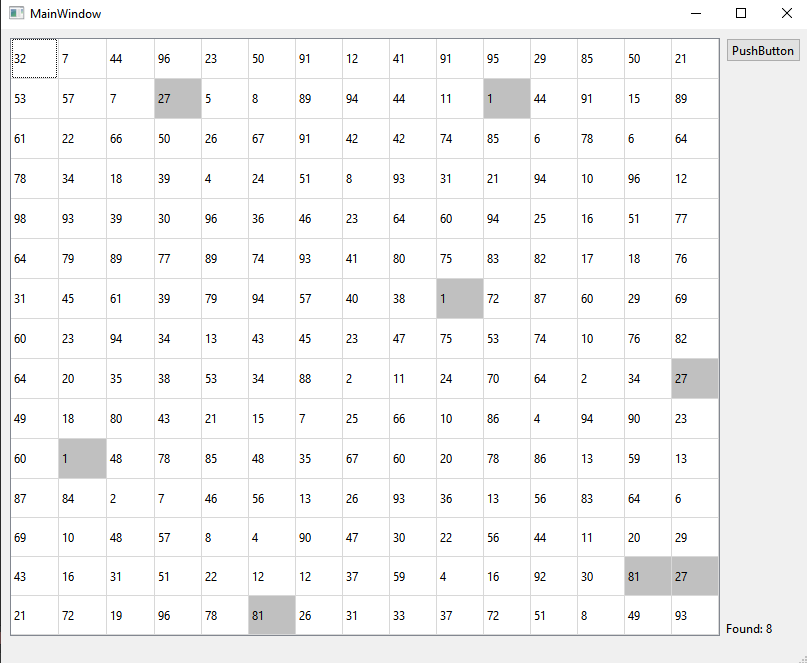
\includegraphics[width=0.6\textwidth]{scr1.PNG}

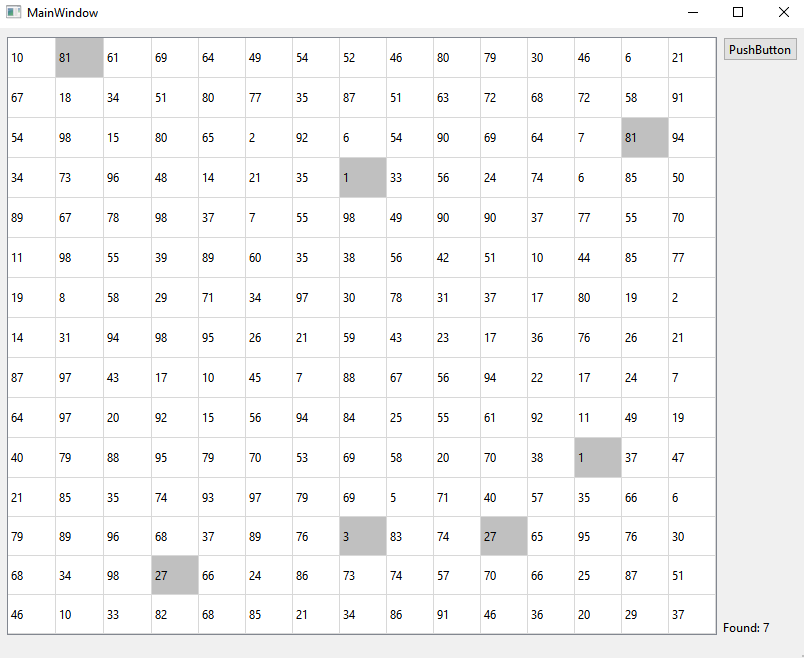
\includegraphics[width=0.6\textwidth]{scr2.PNG}